%%%%%
%%Title: HiPi+Bus V0.2 Chapter 7
%%Creator: Ando Ki
%%CreationDate: April 1992
%%FileName: sec5
%%RelatedFile: ch7
%%%%%
\section{백플레인의 특성}
\subsection{백플레인의 특성임피던스}
백플레인의 버스클럭 신호선의 특성임피던스는 50$\Omega$을 유지해야 하고,
나머지 백플레인 신호선의 특성임피던스는 콘넥터를 꽂기 위한 홀이 없는
상태에서 80$\Omega$이어야 하고,
홀과 콘넥터를 연결하였을때 60$\Omega$ 이상이어야 하고,
모든 슬롯에 보드가 꽂힌 상태에서 20$\Omega$이상을 유지해야 한다.
\subsection{터미네이션}
백플레인에는 두가지 터미네이션 방법을 사용한다.
버스클럭의 경우 [그림~\ref{figure:terminator}.a]과 같이 직렬터미네이션 방법을사용하고,
나머지 신호선들은 [그림~\ref{figure:terminator}.b]과 같이 병렬터미네이션 방법을사용한다.
\begin{figure}[htb]
    \centerline{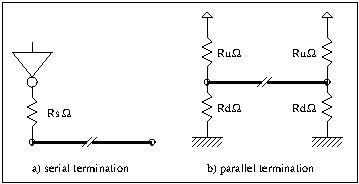
\includegraphics{ch7/FIG/terminator.jpg}}
   \caption{터미네이션 방법}\label{figure:terminator}
\end{figure}
%%%%%
%\end{document}
%%%%%
